%
% ---------------------------------------------------------------
% Copyright (C) 2012-2018 Gang Li
% ---------------------------------------------------------------
%
% This work is the default powerdot-tuliplab style test file and may be
% distributed and/or modified under the conditions of the LaTeX Project Public
% License, either version 1.3 of this license or (at your option) any later
% version. The latest version of this license is in
% http://www.latex-project.org/lppl.txt and version 1.3 or later is part of all
% distributions of LaTeX version 2003/12/01 or later.
%
% This work has the LPPL maintenance status "maintained".
%
% This Current Maintainer of this work is Gang Li.
%
%

\documentclass[
 size=14pt,
 paper=smartboard,  %a4paper, smartboard, screen
 mode=present, 		%present, handout, print
 display=slides, 	% slidesnotes, notes, slides
 style=tuliplab,  	% TULIP Lab style
 pauseslide,
 fleqn,leqno]{powerdot}


\usepackage{cancel}
\usepackage{caption}
\usepackage{stackengine}
\usepackage{smartdiagram}
\usepackage{attrib}
\usepackage{amssymb}
\usepackage{amsmath} 
\usepackage{amsthm} 
\usepackage{mathtools}
\usepackage{rotating}
\usepackage{graphicx}
\usepackage{boxedminipage}
\usepackage{rotate}
\usepackage{calc}
\usepackage[absolute]{textpos}
\usepackage{psfrag,overpic}
\usepackage{fouriernc}
\usepackage{pstricks,pst-3d,pst-grad,pstricks-add,pst-text,pst-node,pst-tree}
\usepackage{moreverb,epsfig,subfigure}
\usepackage{color}
\usepackage{booktabs}
\usepackage{etex}
\usepackage{breqn}
\usepackage{multirow}
\usepackage{natbib}
\usepackage{bibentry}
\usepackage{gitinfo2}
\usepackage{siunitx}
\usepackage{nicefrac}
%\usepackage{geometry}
%\geometry{verbose,letterpaper}
\usepackage{media9}
\usepackage{animate}
%\usepackage{movie15}
\usepackage{auto-pst-pdf}

\usepackage{breakurl}
\usepackage{fontawesome}
\usepackage{xcolor}
\usepackage{multicol}



\usepackage{verbatim}
\usepackage[utf8]{inputenc}
\usepackage{dtk-logos}
\usepackage{tikz}
\usepackage{adigraph}
%\usepackage{tkz-graph}
\usepackage{hyperref}
%\usepackage{ulem}
\usepackage{pgfplots}
\usepackage{verbatim}
\usepackage{fontawesome}


\usepackage{todonotes}
% \usepackage{pst-rel-points}
\usepackage{animate}
\usepackage{fontawesome}

\usepackage{listings}
\lstset{frameround=fttt,
frame=trBL,
stringstyle=\ttfamily,
backgroundcolor=\color{yellow!20},
basicstyle=\footnotesize\ttfamily}
\lstnewenvironment{code}{
\lstset{frame=single,escapeinside=`',
backgroundcolor=\color{yellow!20},
basicstyle=\footnotesize\ttfamily}
}{}


\usepackage{hyperref}
\hypersetup{ % TODO: PDF meta Data
  pdftitle={Presentation Title},
  pdfauthor={Gang Li},
  pdfpagemode={FullScreen},
  pdfborder={0 0 0}
}


% \usepackage{auto-pst-pdf}
% package to show source code

\definecolor{LightGray}{rgb}{0.9,0.9,0.9}
\newlength{\pixel}\setlength\pixel{0.000714285714\slidewidth}
\setlength{\TPHorizModule}{\slidewidth}
\setlength{\TPVertModule}{\slideheight}
\newcommand\highlight[1]{\fbox{#1}}
\newcommand\icite[1]{{\footnotesize [#1]}}

\newcommand\twotonebox[2]{\fcolorbox{pdcolor2}{pdcolor2}
{#1\vphantom{#2}}\fcolorbox{pdcolor2}{white}{#2\vphantom{#1}}}
\newcommand\twotoneboxo[2]{\fcolorbox{pdcolor2}{pdcolor2}
{#1}\fcolorbox{pdcolor2}{white}{#2}}
\newcommand\vpspace[1]{\vphantom{\vspace{#1}}}
\newcommand\hpspace[1]{\hphantom{\hspace{#1}}}
\newcommand\COMMENT[1]{}

\newcommand\placepos[3]{\hbox to\z@{\kern#1
        \raisebox{-#2}[\z@][\z@]{#3}\hss}\ignorespaces}

\renewcommand{\baselinestretch}{1.2}


\newcommand{\draftnote}[3]{
	\todo[author=#2,color=#1!30,size=\footnotesize]{\textsf{#3}}	}
% TODO: add yourself here:
%
\newcommand{\gangli}[1]{\draftnote{blue}{GLi:}{#1}}
\newcommand{\shaoni}[1]{\draftnote{green}{sn:}{#1}}
\newcommand{\gliMarker}
	{\todo[author=GLi,size=\tiny,inline,color=blue!40]
	{Gang Li has worked up to here.}}
\newcommand{\snMarker}
	{\todo[author=Sn,size=\tiny,inline,color=green!40]
	{Shaoni has worked up to here.}}

%%%%%%%%%%%%%%%%%%%%%%%%%%%%%%%%%%%%%%%%%%%%%%%%%%%%%%%%%%%%%%%%%%%%%%%%
% title
% TODO: Customize to your Own Title, Name, Address
%
\title{Air Pollution Prediction based on multicollinearity}
\author{
Shanika Iroshi Nanayakkara
\\Deakin University
}
\date{03/06/2022}


% Customize the setting of slides
\pdsetup{
% TODO: Customize the left footer, and right footer
rf=\href{http://www.tulip.org.au}{
Last Changed by: \textsc{Shanika}\ \gitVtagn-\gitAbbrevHash\ (\gitAuthorDate)
},
cf={Air Pollution Prediction},
}


\begin{document}

\maketitle

%\begin{slide}{Overview}
%\tableofcontents[content=sections]
%\end{slide}


%%==========================================================================================
%%
\begin{slide}[toc=,bm=]{Overview}
\tableofcontents[content=currentsection,type=1]
\end{slide}
%%
%%==========================================================================================


\section{Problem Definition}


%%==========================================================================================
%%
\begin{slide}{Air pollution predictors}
\begin{center}
\twotonebox{\rotatebox{90}{Defn}}{\parbox{.86\textwidth}
{Predict air pollution composition in atmosphere in the future.
\begin{itemize}
\item Use predictors such as \textcolor{orange}{Temperature},\textcolor{orange}{Humidity},\textcolor{orange}{Sensor data}.
\item Response variables are \textcolor{orange}{carbon monoxide},\textcolor{orange}{benzene},\textcolor{orange}{ notrous oxide}
\end{itemize}
}}

\end{center}


%%==========================================================================================
\begin{note}
First, I will introduce the problem definition.
In the real life,
a teacher may be interested in the characteristics that
make one student obvious different from others.
Or,
NBA sports coaches would prefer to
know the advantages and disadvantages of one player.
Here, the player can be regarded as a query object.

For example, team A has five players,
each player has four features.
The NBA sports coaches may want to know the features of
player $1$ that are different from others.

The above example can be seen as outlying aspects mining.
The main purpose of outlying aspects mining is to identify
the outstanding features of the query object.
\end{note}
%%==========================================================================================

\end{slide}
%%
%%==========================================================================================


%%==========================================================================================
%%
\begin{slide}[toc=,bm=]{Linear Regression vs Rigid Regrssion}
\begin{center}

\end{center}

\bigskip

\twocolumn[
\savevalue{lfrheight}=8.6cm,
\savevalue{lfrprop}={
linestyle=solid,framearc=.2,linewidth=1pt},
rfrheight=\usevalue{lfrheight},
rfrprop=\usevalue{lfrprop}
]{
Linear Regression
\begin{itemize}
\item
\smallskip
Linear regression presents relationship as a straight line. 
\smallskip
\item
\smallskip
Show correlation between two variables (one predictor for response variable/variables).
\smallskip
\item 
\smallskip
Response should be continuous and independent variable(s) (predictor variables) can be continuous or discrete.
\smallskip
\end{itemize}
}{
Rigid Linear Regression
\begin{itemize}
\item
\smallskip
Use to implement multicollinearity
of predictor variables which are highly correlated each other
\textcolor{orange}{objects} in the whole dataset.
\smallskip
\item
\smallskip
Add penalty values to reduce the loss or error of
linear regression cause by bias and/or variance of the variables.
\end{itemize}
}

%%==========================================================================================
%%==========================================================================================

\end{slide}
%%
%%==========================================================================================


%%=================================================

\section{Challenges}




%%==========================================================================================
%%
\begin{slide}[toc=,bm=]{Challenges}
\twocolumn
{
multicollinearity
\begin{itemize}
\item
\smallskip
Focus on correlation between \textcolor{orange}{predictors}.

\end{itemize}
%\vspace{0.75cm}
%\vspace{0.1cm}
\begin{figure}
  \centering
  \selectcolormodel{rgb}
 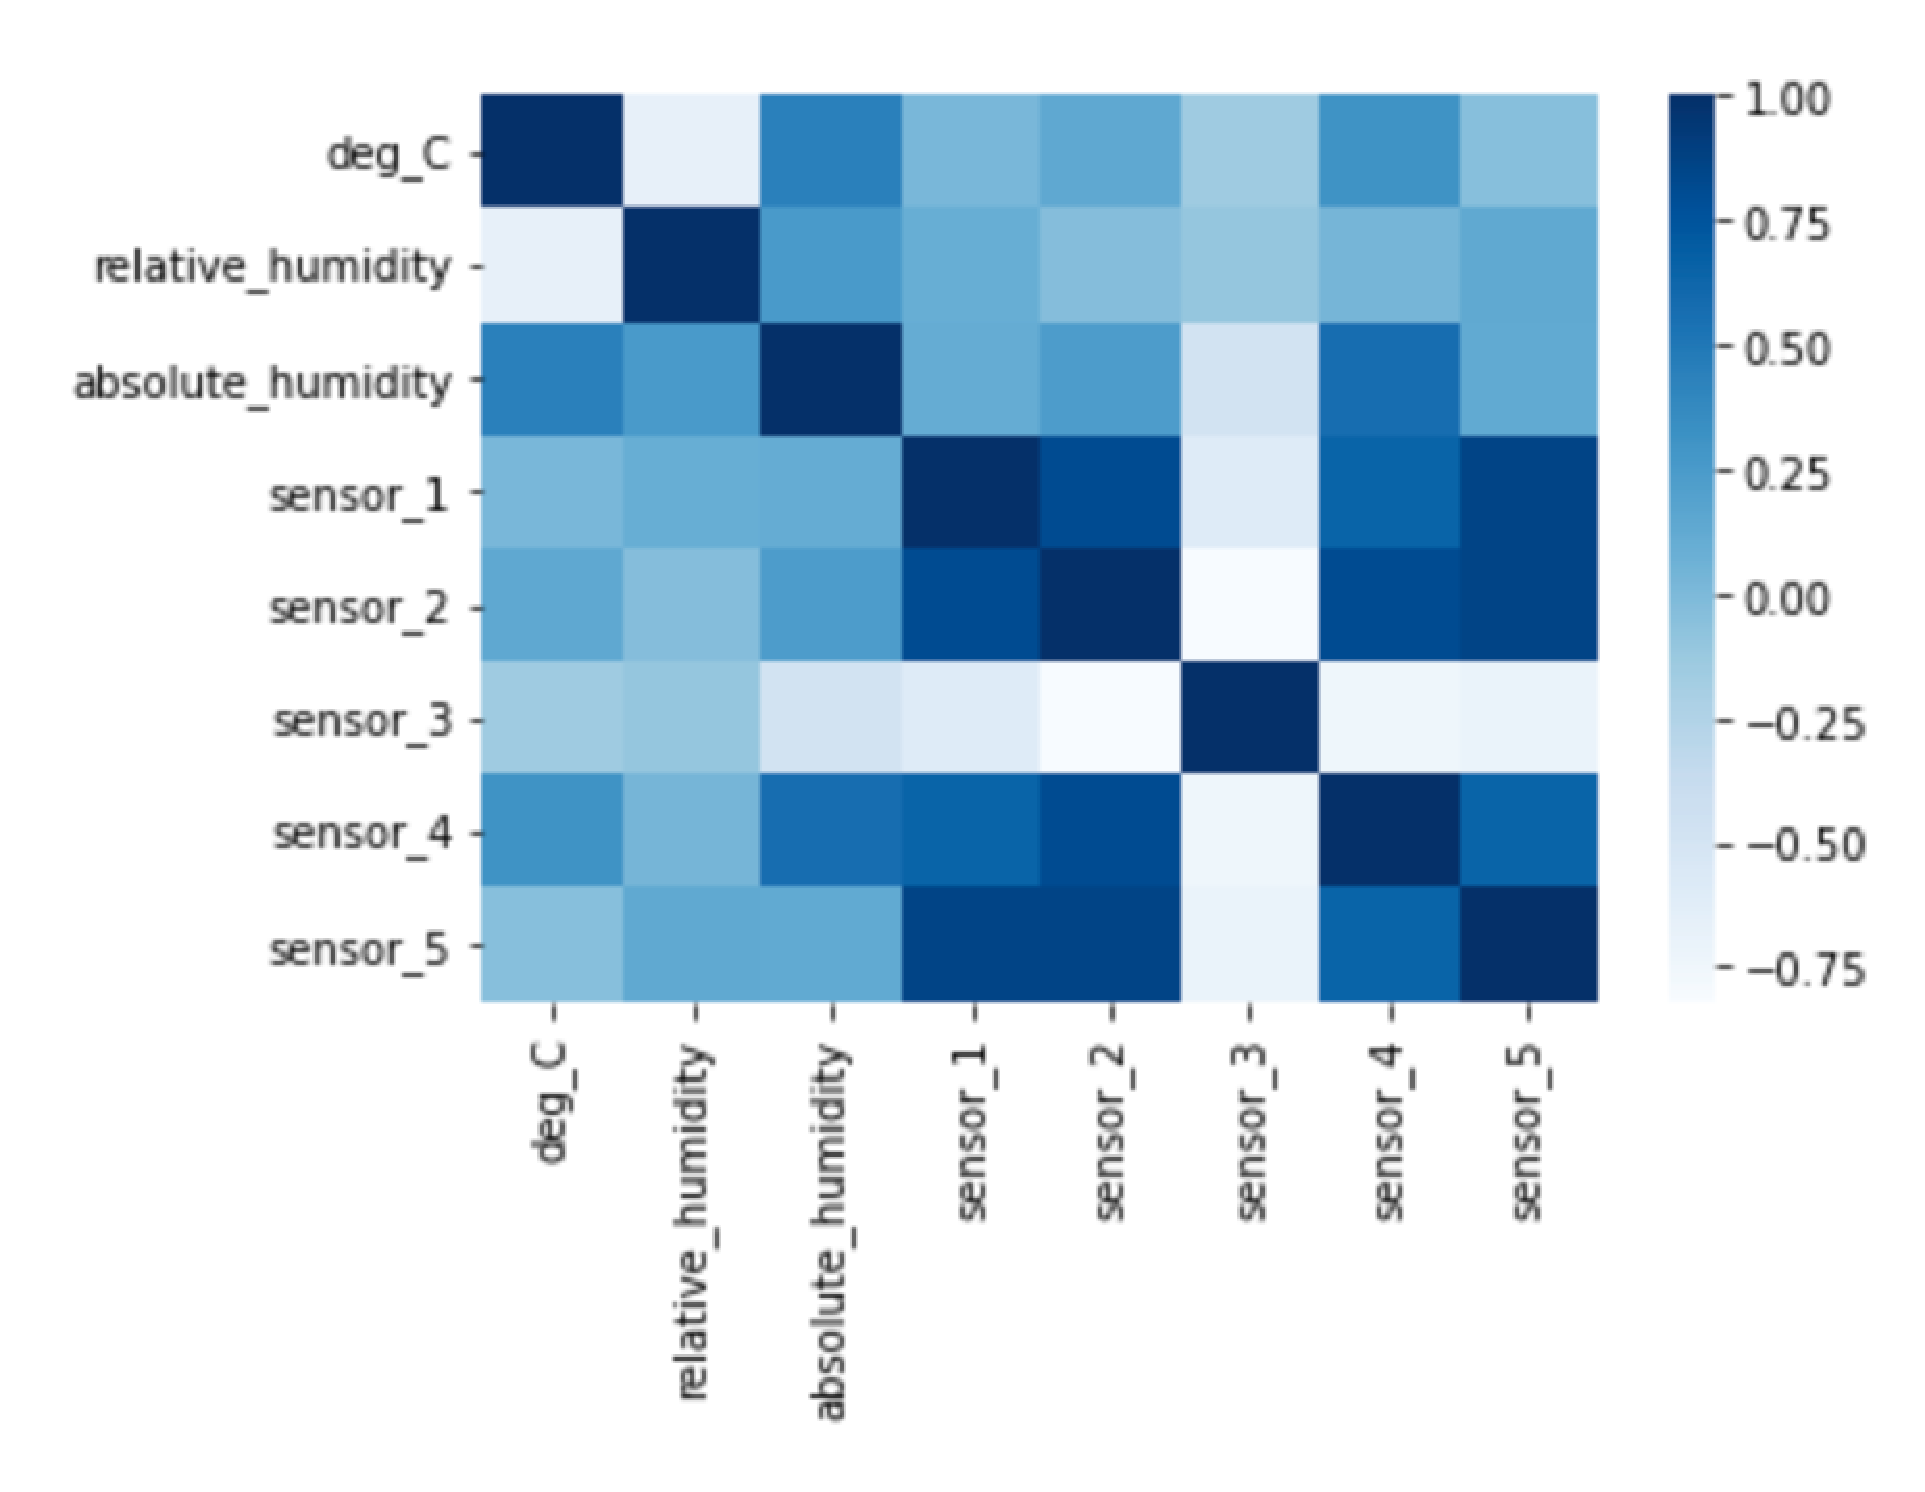
\includegraphics[width=1.0\linewidth,height=0.8\linewidth]{graphics//Fig_heatmap.eps}
  \caption{Framework of Model} \label{Heatmap}
\end{figure}
}
{
    
    Reasons for \textcolor{orange}{multicollinearity} in predictors.
    
    \begin{itemize}
    \item
    Inaccurate use of different types of variables.
    \item
    Poor selection of questions or null hypothesis.
    \item Variable repetition.
    \item A dependent variable selection.
    \item High correlation.
    \item Use of dummy variables.
   
    \end{itemize}
}

%%==========================================================================================

\end{slide}
%%
%%==========================================================================================


%%==========================================================================================
%%
\begin{slide}{Challenges}
%Challenges (1)

Fixing \textcolor{orange}{multicollinearity}

\begin{itemize}
\item
Obtain more data.
\item
Utilize a ridge regression.
\item Utilize a partial squares regression
\item Removing a variable.
\item Do nothing.
\end{itemize}


%%==========================================================================================
%%==========================================================================================

\end{slide}
%%
%%==========================================================================================


%%==========================================================================================

\section{Proposed Model}


%%==========================================================================================
%%
\begin{slide}[toc=,bm=]{}

Framework of Proposed Model:

%\begin{center}
  %\includegraphics[width=1.0\linewidth,height=.4\linewidth]{C:/Users/lenovo/Desktop/slide picture/fare.eps}\
   % {image1:fare frequency}\
%\end{table}

\begin{figure}
  \centering
  \selectcolormodel{rgb}
 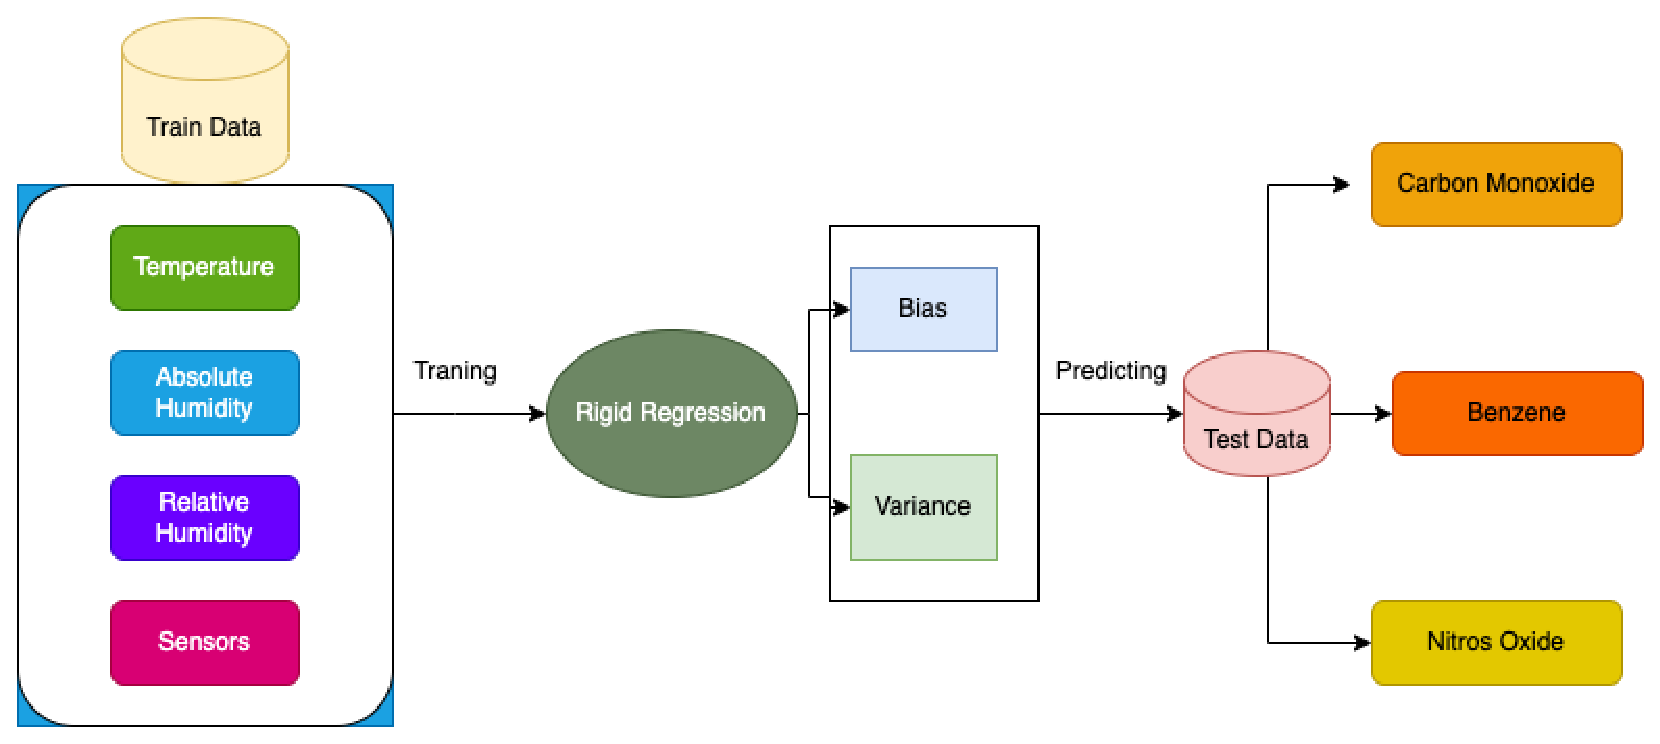
\includegraphics[width=1.0\linewidth,height=.4\linewidth]{graphics//Air Prediction.eps}
  \caption{Framework of Model} \label{framework}
\end{figure}

\end{slide}
%%
%%==========================================================================================


%%==========================================================================================

%%==========================================================================================

%%
\begin{slide}[toc=,bm=]{Preprocessing and Model training}
  \twocolumn
  {
  Bias and Variance

  %\vspace{0.75cm}
  %\vspace{0.1cm}
  \begin{figure}
    \selectcolormodel{rgb}
    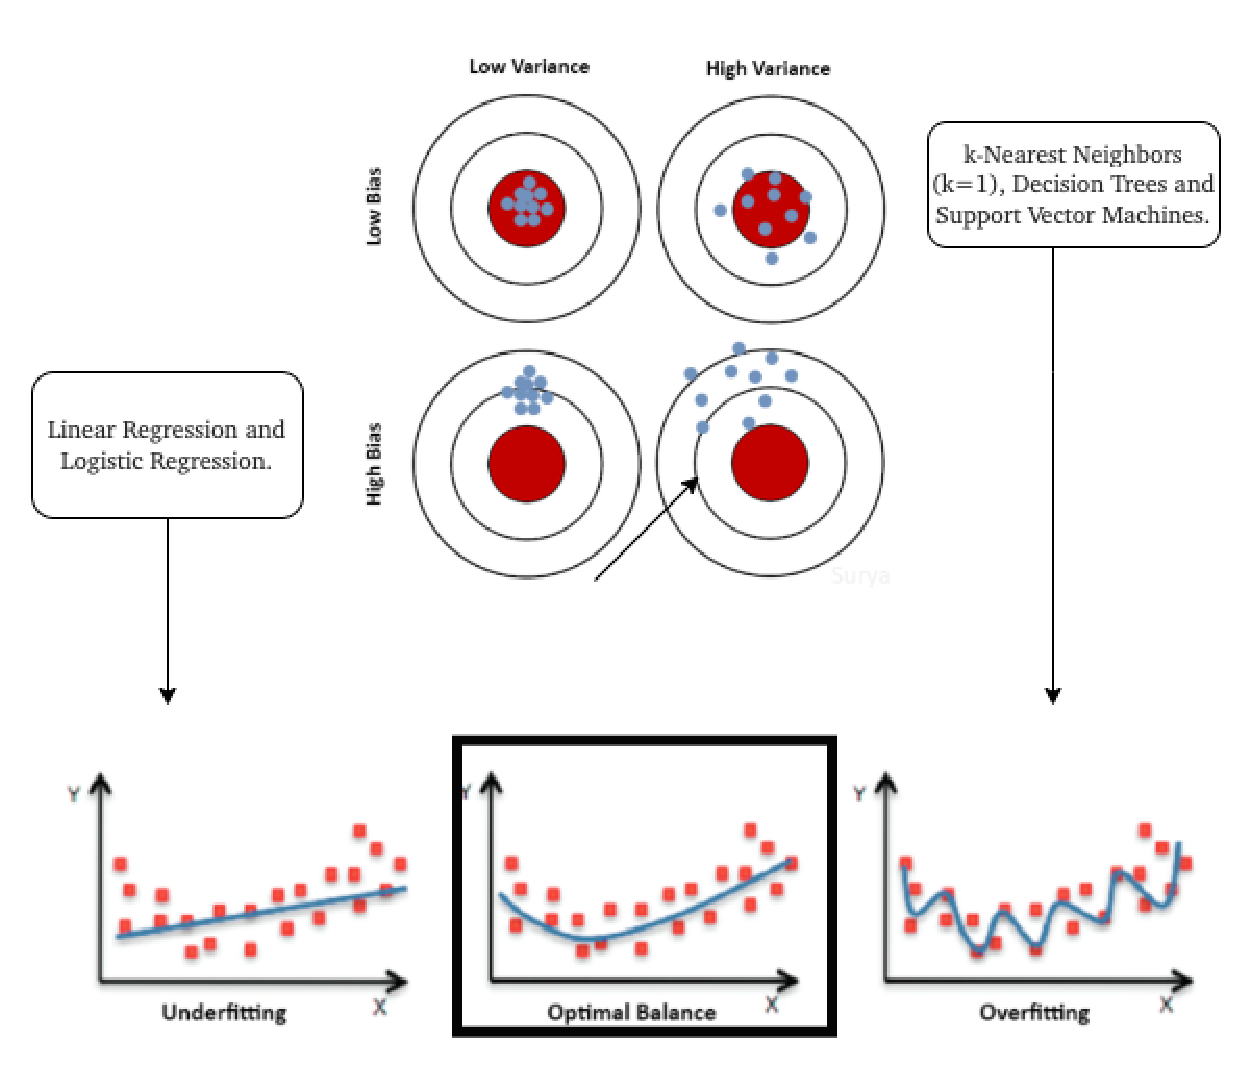
\includegraphics[width=0.8\linewidth,height=0.8\linewidth]{graphics//Bias_and_VrarianceAll.eps}
    \caption{Bias and VAriance} \label{Bias}
 \end{figure}
  }
  {
      
      Reasons for \textcolor{orange}{multicollinearity} in predictors.
      
      \begin{itemize}
      \item Remove Duplicates.
      \item Remove unwanted columns.
      \item Scale for data consistency.
      \item Remove Outliers.
      \end{itemize}
  }
  

  
  \end{slide}


%%
\begin{slide}[toc=,bm=]{Preprocessing and Model training}
  
  {
 

  %\vspace{0.75cm}
  %\vspace{0.1cm}

  }
  {
    \begin{figure}
      \selectcolormodel{rgb}
      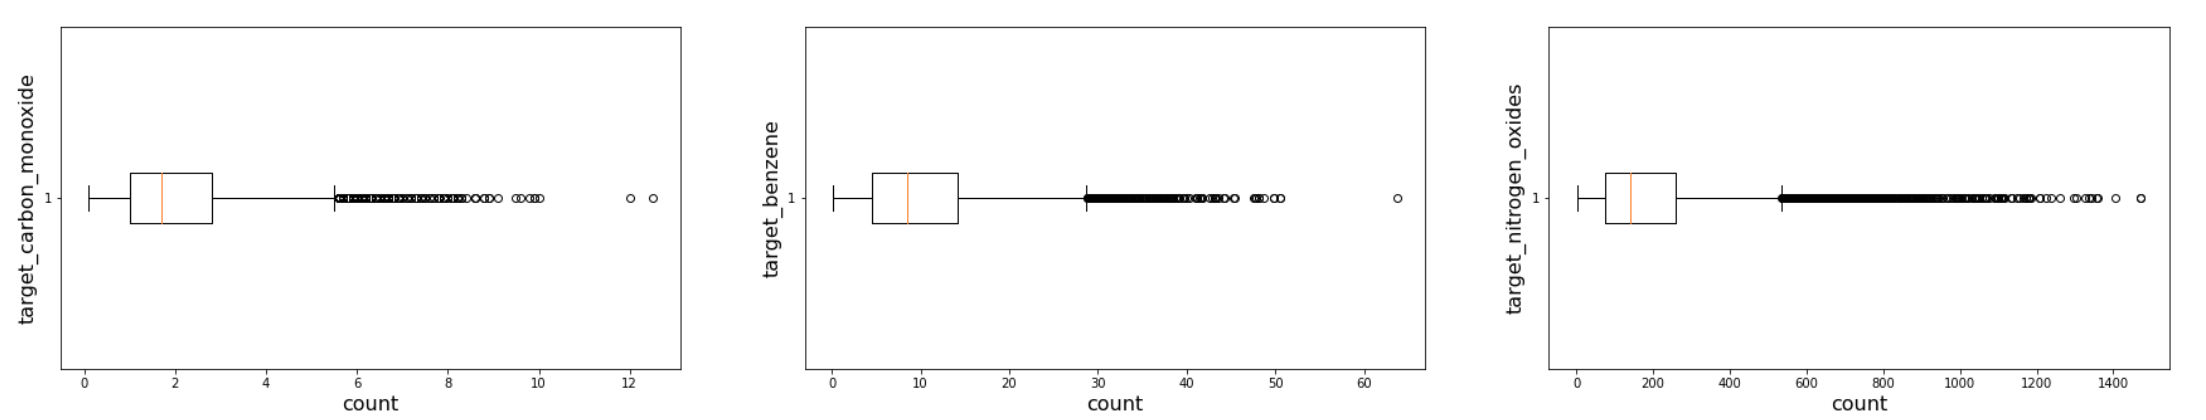
\includegraphics[width=1.0\linewidth,height=0.4\linewidth]{graphics//Fig_Boxplot.eps}
      \caption{Response data distribution and Outlier Detection.} \label{Bias}
   \end{figure}
  }
  

  
  \end{slide}
%%============================================================================

\begin{slide}{ Model Prediction and Evaluation}
  %Step Three - Outlying Aspects Identification
  \begin{itemize}
  \item
  Relationships between predictors and response variables over time.
  
  \end{itemize}
  
  
  \begin{figure}
    \selectcolormodel{rgb}
    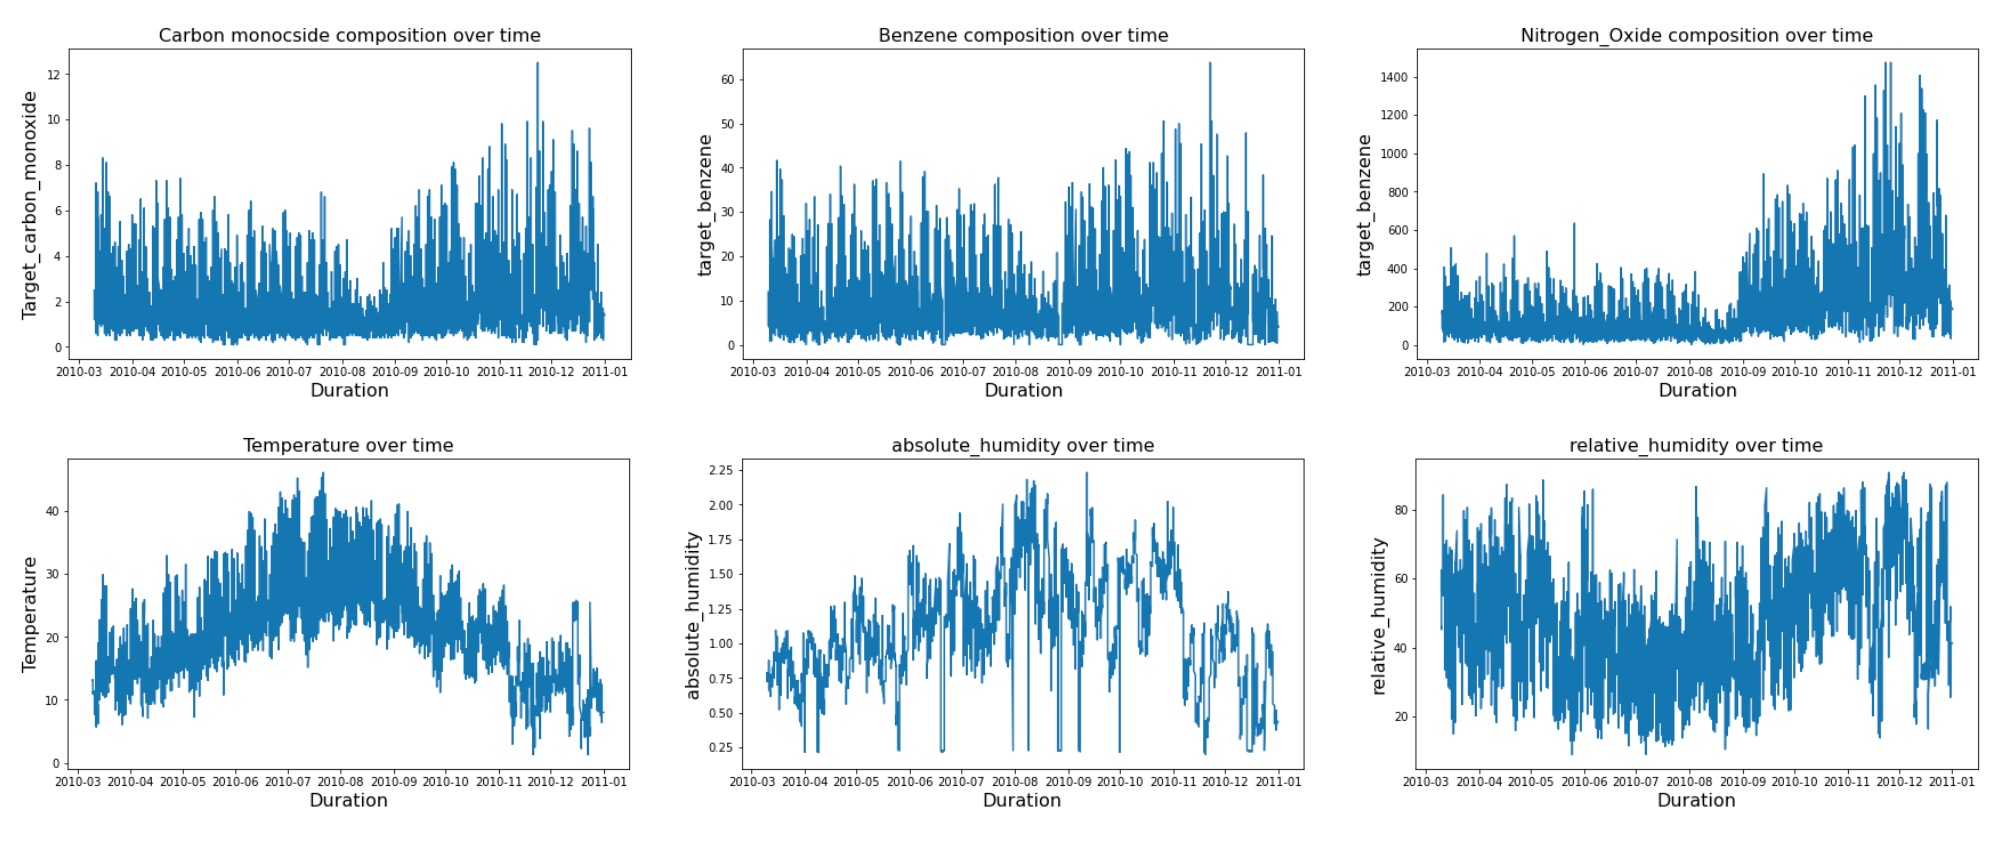
\includegraphics[width=0.9\linewidth,height=0.5\linewidth]{graphics//Fig_Correlations.eps}
    \caption{Relationships over the time} \label{Bias}
  \end{figure}
  \end{slide}
%%
\begin{slide}{ Model Prediction and Evaluation}
%Step Three - Outlying Aspects Identification
\begin{itemize}
\item
Determination of coefficient.

\end{itemize}


\begin{figure}
  \selectcolormodel{rgb}
  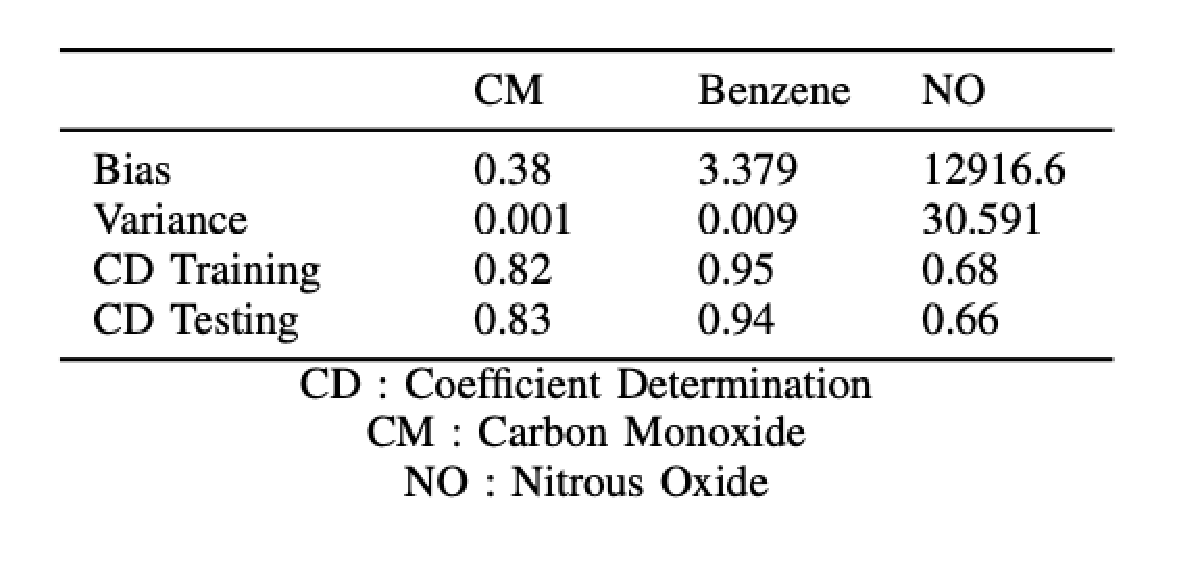
\includegraphics[width=0.9\linewidth,height=0.4\linewidth]{graphics//Evaluation.eps}
  \caption{performance Evaluation} \label{Bias}
\end{figure}
\end{slide}
%%
%%=================================================

%%==========================================================================================


%%==========================================================================================


%%
%%==========================================================================================



\section{Evaluation Results}

\begin{slide}[toc=,bm=]{Evaluation}
\begin{figure}[htbp]
  \centering
  \subfigure[Carbon_monoxide_prediction]{
      \selectcolormodel{rgb}
      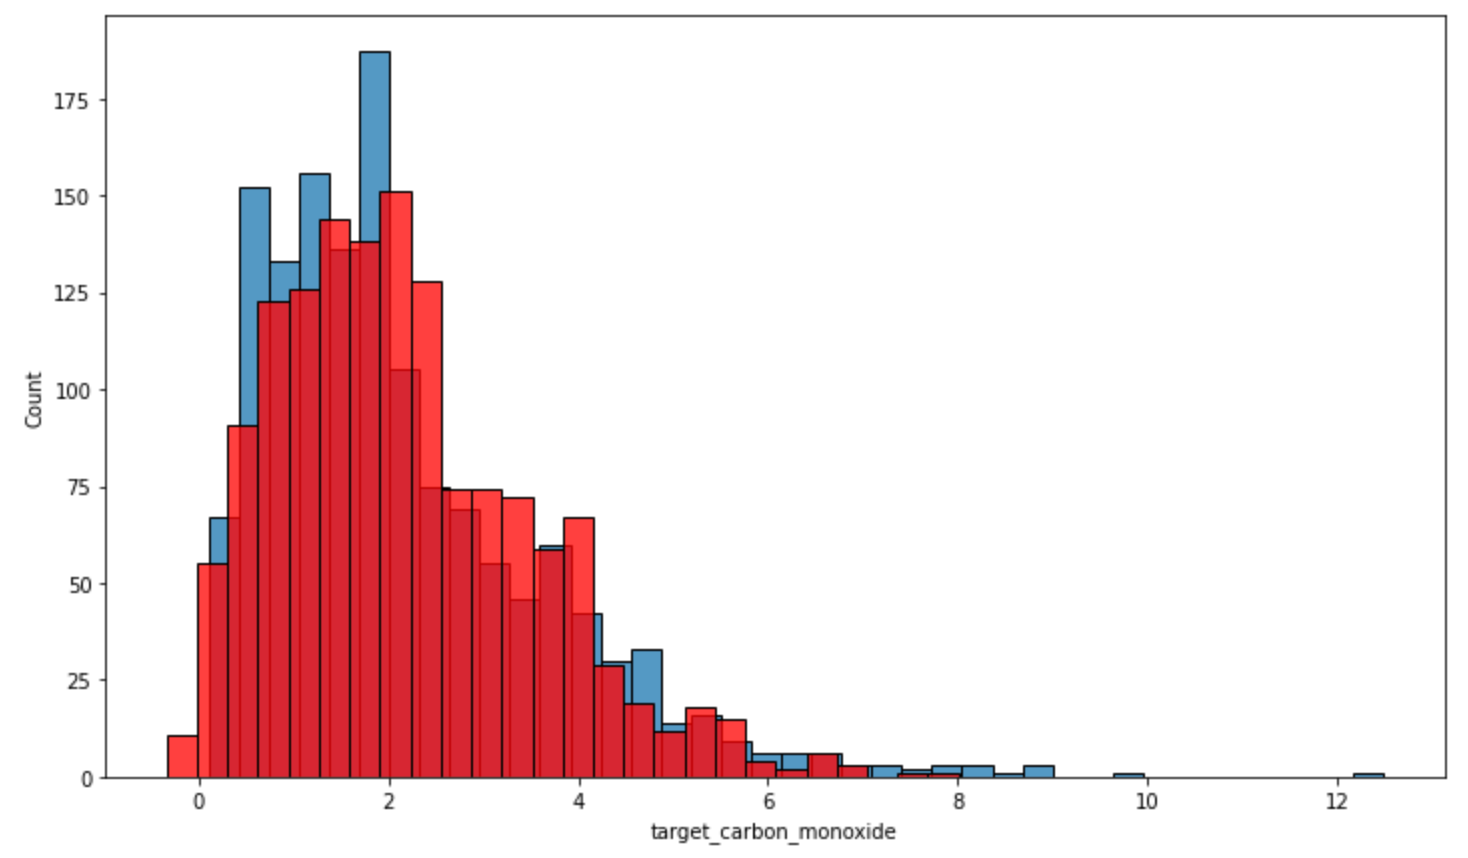
\includegraphics[width=0.3\linewidth,height=.3\linewidth]{graphics//Fig_CM_ModelAccuracy.eps}
      \label{fig:fre-dis-f1}
  }
  \subfigure[Benzene_Prediction]{
      \selectcolormodel{rgb}
      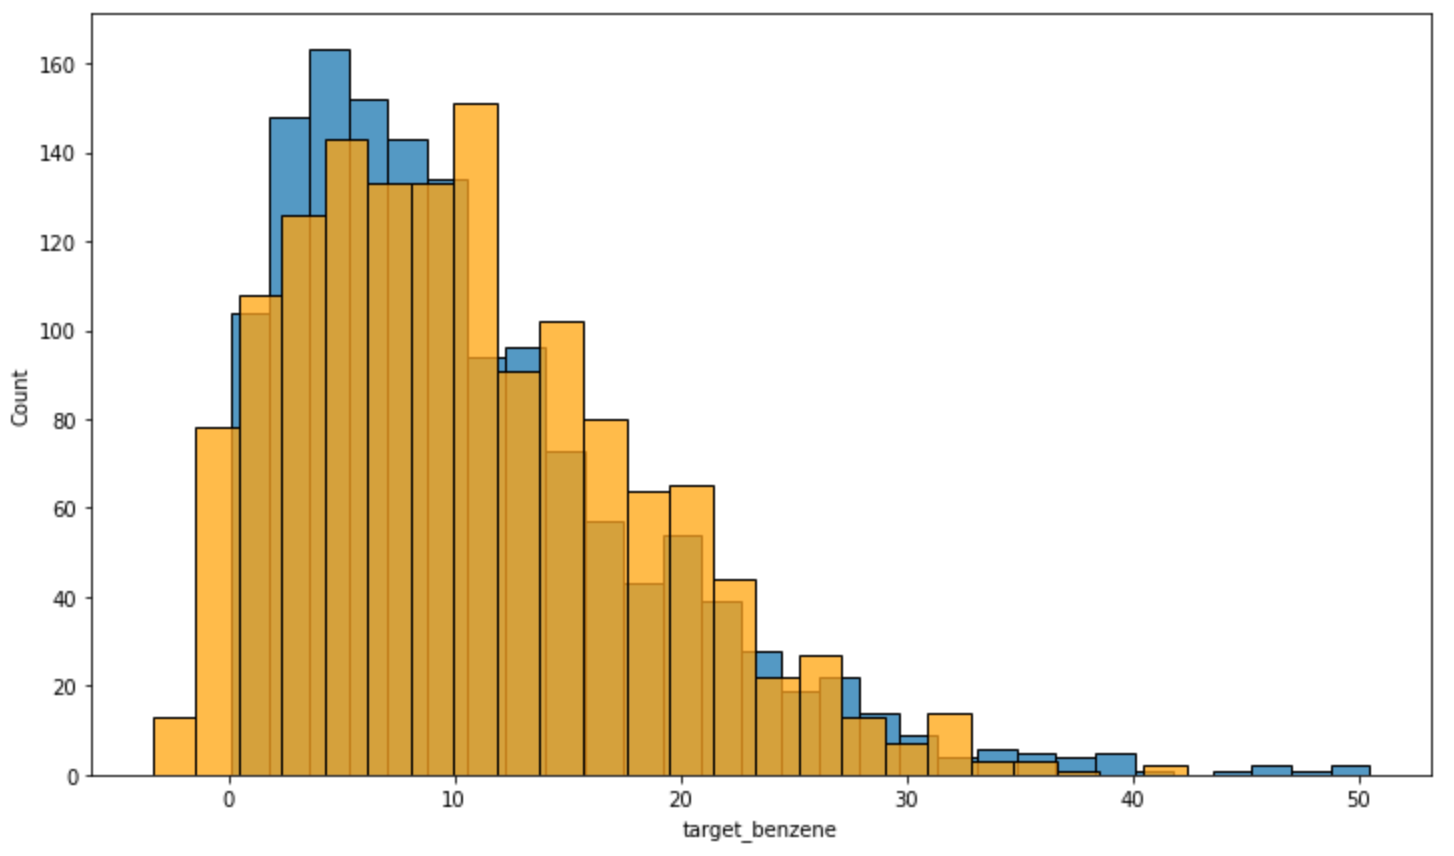
\includegraphics[width=0.3\linewidth,height=.3\linewidth]{graphics//Fig_BenzeneModelBehavior.eps}
      \label{fig:fre-dis-f2}
  }
  \subfigure[Nitrous Oxide Prediction]{
      \selectcolormodel{rgb}
      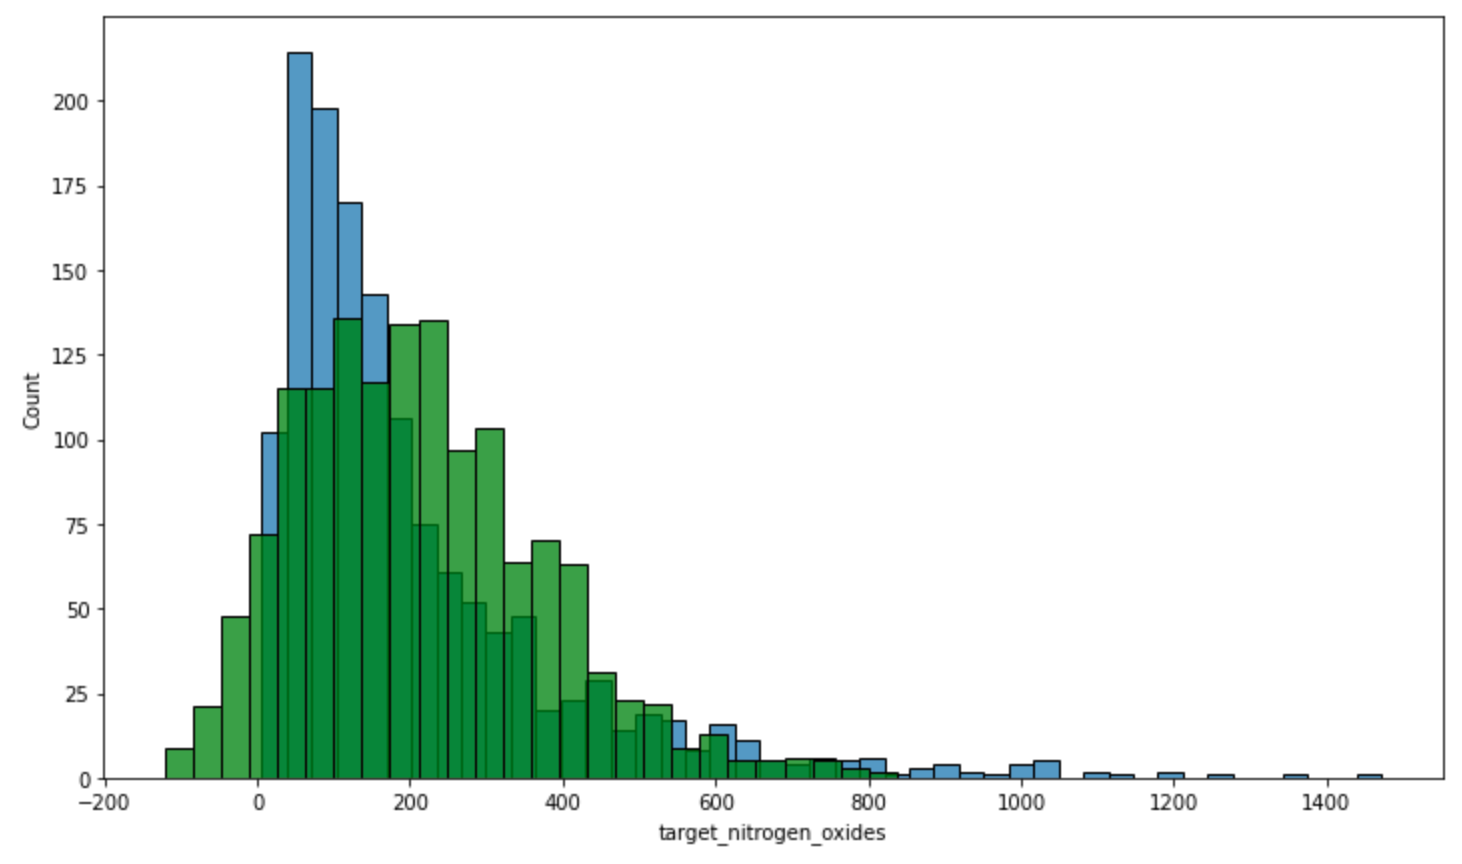
\includegraphics[width=0.3\linewidth,height=.3\linewidth]{graphics//Fig_NOxModelBehavior.eps}
      \label{fig:fre-dis-f3}
  }
  \caption{Histogram of three test feature predictions}
  \label{fig:fre-dis-each-feature}
\end{figure}

\end{slide}
\section{Conclusion}

%%==========================================================================================
%%
\begin{slide}[toc=,bm=]{Conclusion}
\begin{itemize}
\item
\smallskip
Problem Definition: we propose prediction model to predict air pollution compo-
nents which are specified as carbon monoxide, benzene and nitrous oxide.
Algorithm Consequently, we use rigid linear regression instead general linear re-
gression method.


\item
\smallskip
Strategies :We uses multiple predictors such as temperature, absolute and relative
humidity and five sensor data. We identify that these predictors are correlated
among each other. Therefore, we reveals the need of handling multicollinearity.
We clearly show the performance efficiency of proposed models using determi-
nation of coefficient, bias and variance scores for each models.

\item
\smallskip
Recommendations : Evaluate how well these prediction models behave on adding
more noisy data. How to affect prediction accuracy by noisy data. Increase the
amount of predictors to predict air pollution

\end{itemize}

%%==========================================================================================
\begin{note}
In conclusion,
we firstly formalized the problem of
group outlying aspects mining,

Then proposed a novel method GOAM algorithm to address the problem of
group outlying aspects mining,
and the proposed method use pruning to reduce time complexity
while identifying the suitable set of outlying features for the interested group.

Thank you and any question?
\end{note}
%%==========================================================================================

\end{slide}
%%
%%==========================================================================================


%%==========================================================================================
%
\begin{slide}[toc=,bm=]{Questions?}
\begin{center}
\begin{figure}
    \animategraphics[autoplay, loop, height=0.4\textheight]{5}{./graphics//gif//question//q_}{1}{30}
\end{figure}
\end{center}
\end{slide}
%%
%%==========================================================================================


%%==========================================================================================
% TODO: Contact Page
\begin{wideslide}[toc=,bm=]{Contact Information}
\centering
\vspace{\stretch{1}}
\twocolumn[
lcolwidth=0.35\linewidth,
rcolwidth=0.65\linewidth
]
{
% \centerline{
\includegraphics[scale=.2]{tulip-logo.eps}}
}
{
\vspace{\stretch{1}}
Associate Professor Gang Li\\
School of Information Technology\\
Deakin University, Australia
\begin{description}
 \item[\textcolor{orange}{\faEnvelope}] \href{mailto:gangli@tulip.org.au}
 {\textsc{\footnotesize{gangli@tulip.org.au}}}

 \item[\textcolor{orange}{\faHome}] \href{http://www.tulip.org.au}
 {\textsc{\footnotesize{Team for Universal Learning and Intelligent Processing}}}
\end{description}
}
\vspace{\stretch{1}}
\end{wideslide}

\end{document}

\endinput
